\section{Model construction}\label{lca}
%%%%%%%%%%%%%%%%
\subsection{Unigram and mixture of unigram model}
Before intrducing Topic-word Model,Let us review some basic model for short test.
$N$ represents the number of words in the document to be generated, $w_n$ represents the $n$th word $w$ generated, and $p(w)$ represents the distribution of the word $w$, which can be obtained through statistical learning of the corpus, such as giving a book to count each word in The probability of occurrence in the book.The whole test can be represented by Vector $W = (w_1,w_2,\dots,w_n)$.
We assume that words are independent of each other, so that the probability that this document will be generated is:
\begin{eqnarray*}
p(W) &=& p(w_1,w_2,\dots,w_n) \\
    &=& p(w_1)p(w_2)..p(w_n)
\end{eqnarray*}
As mentioned in section of Preliminaries,each text can be converted into a vector $N=(n_1,n_2,\dots,n_V)$ by Bag of Word model and V is number of Vocabulary.
We further assume that the text matrix is subject to a multinomial distribution.
\[
  p(w_1)p(w_2)..p(w_n) = \prod_{k=1}^V p_k^{n_k}
\]


The disadvantage of the method of the unigram model is that there are no relationship between the word in  the document and it is hard to inference the distriution of word in defferent documents with different topic. The mixture of unigram\cite{tcf} method improves it by introducing topic for each document. The model samples a topic from distribution $p(z)$ before generating each word.
\[
  p(W|Z) = \sum_zp(z)\prod_{n=2}^{N}p(w_n|z)
\]
$z$ represents a topic, $p(z)$ represents the probability distribution of the theme, $z$ is generated by $p(z)$ according to probability; $ p(w|z)$ represents the distribution of $w$ given $z$, which can be regarded as a $k * V$ matrix, $k$ is the number of topics, $V$ is the number of words, each line represents the probability distribution of words corresponding to this topic, that is, the probability of each word contained in topic $z$, generated by this probability distribution with a certain probability.

\subsection{Probabilistic Latent Semantic Analysis}
Another widely used topic model is pLSA model. pLSA is a topic model, which is a method of modeling the hidden topics in the text. PLSA means that after the document $d$ is given, the topic $z$ corresponding to the document needs to be selected with a certain probability, and then the word $w$ is selected from the topic $z$ with a certain probability\cite{plsa}.

\begin{figure}
  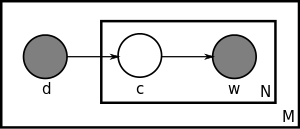
\includegraphics[width=\linewidth]{plsa.png}
  \caption{pLSA model}
  \label{fig:boat1}
\end{figure}

PLSA models the joint distribution of d and w by the following formula:
\[
  p(d,w_n) = p(d)\sum_{k=1}^{K}p(w_n|z)p(z|d)
\]

\begin{enumerate}
  \item Choose a document with probability $p$;
  \item Get the topic $z$ by with probability $p(z|d)$;
  \item Generate a word with probability $p(w_n|z_k)$;
\end{enumerate}}


Imagine that we wants to write $N$ documents, and we needs to determine the word in each position in each document. Suppose we has $K$ optional topics and $V$ optional words. Therefore, we made $K$ dice with $V$ sides, each corresponding to a topic, and each side of the dice corresponds to The selected term. Then, each time a document is written, a K-sided document-topic dice will be made; each time a word is written, the dice will be thrown to select the topic; after the result of the theme is obtained,we can get words by tossing the corresponding topic-word dice. Repeating this method N times, then finish writing all documents

It is easy to find that for a new document, we cannot know what its corresponding $P(d)$. Although the PLSA model is a generative model on a given document, it cannot generate a new unknown document.Another problem with this model is that as the number of documents increases, the parameters of $P(z|d)$ also increase linearly, which leads to the problem of overfitting the model no matter how much training data there is. These two points have become two major flaws that limit the more widespread use of the PLSA model.
